\begin{figure}[h]
\centering
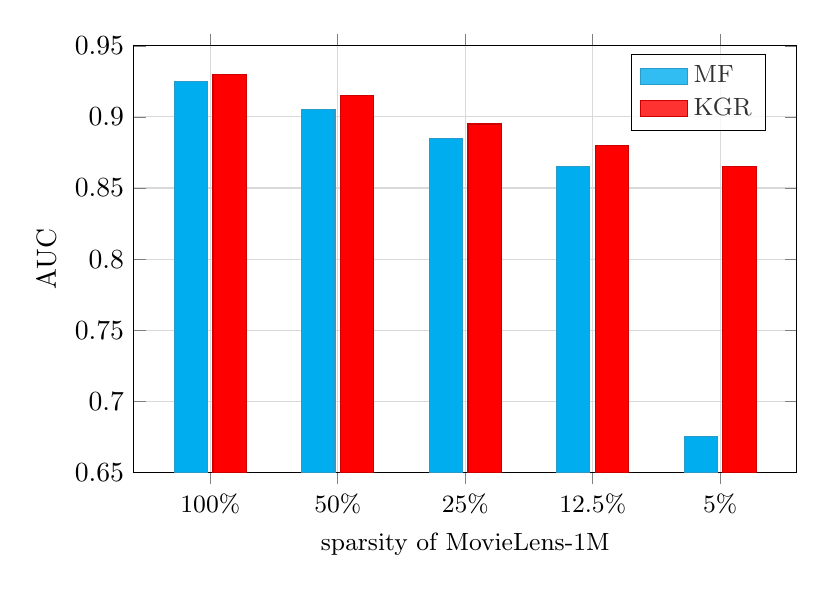
\begin{tikzpicture}
\begin{axis}[
    ybar,
    width=10cm,
    height=7cm,
    ylabel={AUC},
    ymin=0.65,
    ymax=0.95,
    ytick={0.65, 0.70, 0.75, 0.80, 0.85, 0.90, 0.95},
    symbolic x coords={100\%, 50\%, 25\%, 12.5\%, 5\%},
    xtick=data,
    x tick label style={font=\small},
    bar width=12pt,
    legend style={at={(0.75,0.98)}, anchor=north west, font=\small, fill=white, fill opacity=0.8, draw=black},
    legend cell align={left},
    area legend,
    grid=major,
    grid style={gray!30},
    enlarge x limits=0.15,
    xlabel={sparsity of MovieLens-1M},
    xlabel style={font=\small},
]
% MF method (cyan bars)
\addplot[fill=cyan, draw=cyan!80!black] coordinates {
    (100\%, 0.925)
    (50\%, 0.905)
    (25\%, 0.885)
    (12.5\%, 0.865)
    (5\%, 0.675)
};
% KGR method (red bars)
\addplot[fill=red, draw=red!80!black] coordinates {
    (100\%, 0.930)
    (50\%, 0.915)
    (25\%, 0.895)
    (12.5\%, 0.880)
    (5\%, 0.865)
};
\legend{MF, KGR}
\end{axis}
\end{tikzpicture}
\caption{Knowledge-grounded regression (KGR) benchmarking against matrix factorization (MF). Higher AUC is better. Measurements from article \parencite{chen2021collaborative}.}
\label{fig:movielens_auc_sparsity}
\end{figure}